\documentclass[10pt]{beamer}
\usetheme{Pittsburgh}

\usepackage{graphicx}
\usepackage[linesnumbered,ruled,vlined]{algorithm2e}
\usepackage{color,soul}
\usepackage[utf8]{inputenc}
\usepackage[T1]{fontenc}
\usepackage{textcomp}
\usepackage{amsmath, amssymb}
\usepackage{caption}
\usepackage{listings}
\usepackage[italian]{babel}

% figure support
\usepackage{tikz}
\usetikzlibrary{calc}
\usepackage{import}
\usepackage{xifthen}
\usepackage{pdfpages}
\usepackage{transparent}
\usepackage[]{hyperref}
\usepackage{multirow}

% provides the H option
\usepackage{float}

% provides subcaptions
\usepackage{subcaption}

% provides justification
\usepackage{ragged2e}
\justifying

% for logo
\usepackage[export]{adjustbox}

\pdfsuppresswarningpagegroup=1
\setcounter{tocdepth}{1}
\AtBeginSection[]
{
  \begin{frame}<beamer>
    \tableofcontents[currentsection,depth=1]
  \end{frame}
}

\author{Augello Andrea \and Castiglione Francesco Paolo \and La Martina Marco}
\institute{Università degli studi di Palermo}
\begin{document}
\title[Chang'e]{Documentazione - Progetto di Robotica}
	\begin{frame}
		\titlepage
		\begin{figure}[htpb]
			
\includegraphics[width=0.2\textwidth,left]{./img/logo_unipa.png}
		\end{figure}
		
		
	\end{frame}


	\section{Introduzione}\label{sec:Introduzione}
	\frame{\sectionpage}
	\frame{
		La pandemia del coronavirus SARS-CoV-2 ha dato una forte
		spinta alla ricerca sia nel campo sanitario che informatico, mettendo in
		evidenza forti carenze dal punto di vista infrastrutturale.
		
		
		Al momento, considerando la limitata disponibilità del vaccino alle masse, uno dei miglior modi di evitare la contrazione del coronavirus è
		di evitarne l'esposizione. Il distanziamento sociale si configura di
		conseguenza come un prerequisito per una significativa riduzione del numero
		di infetti, come evidenziato da simulazioni di un sistema ad agenti
		\cite{silva2020covid}. Un problema chiave si configura di conseguenza come
		il controllo del rispetto delle norme di distanziamento all'interno degli
		spazi chiusi. 
	}

	\begin{frame}{Obbiettivo}
	L'obbiettivo del progetto è quello di sviluppare un robot con lo scopo di \textbf{evitare assembramenti in ambienti indoor} e di invitare a \textbf{rispettare le norme sul distanziamento sociale}. 
	
	Nella dimostrazione presentata il nostro robot rileva le persone nella stanza e individua i possibili assembramenti. In seguito alla fase di rilevazione si sposterà verso l'assembramento evitando gli ostacoli e, arrivato, esorterà le persone al rispetto del distanziamento sociale.
	\end{frame}
	
	\begin{frame}{Stato dell'arte}
	Un robot che si occupa di far rispettare il distanziamento sociale è quello
	proposto nell'articolo~\cite{sathyamoorthy2020covidrobot}. Sono stati usati
	un TurtleBot 2, una camera RGB-D e CCTV per il rilevamento degli
	assembramenti, una camera termica per rilevare la temperatura corporea e un
	lidar 2-D per evitare le collisioni.
	
	Un altro esempio è quello proposto nell'articolo~\cite{fan2020autonomous}.
	In questo caso sono state usate 2 camere e CCTV per il rilevamento degli
	assembramenti e un lidar 3-D per evitare le collisioni.
	
	\begin{figure}[H]
		\begin{subfigure}{0.49\textwidth}
			\centering
			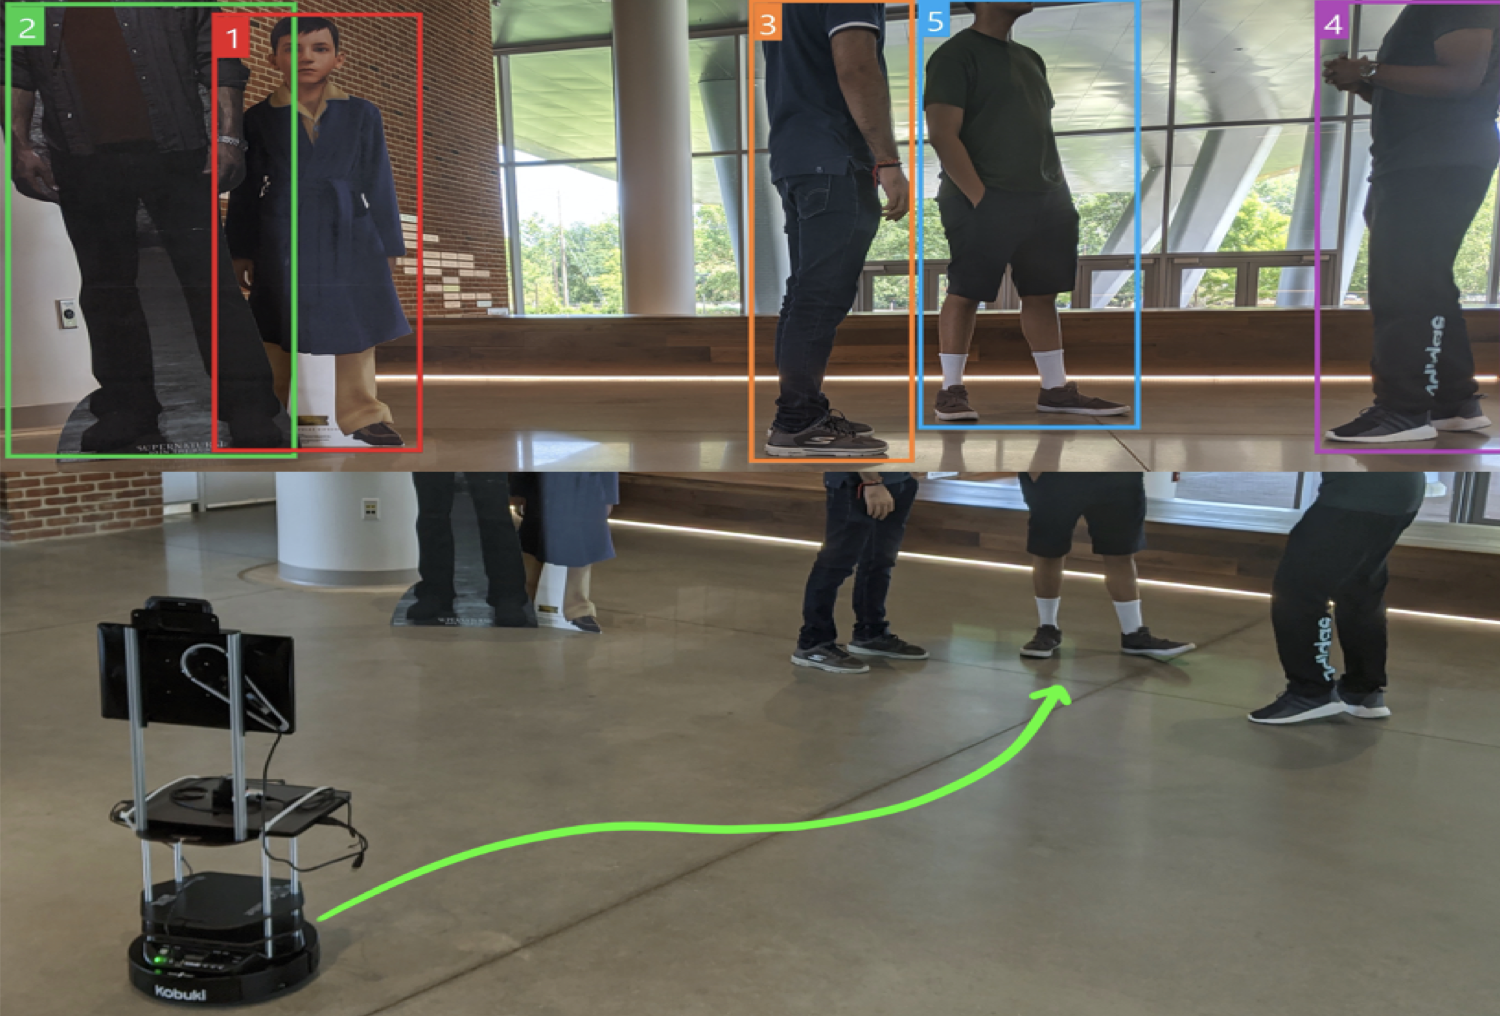
\includegraphics[width=0.8\linewidth]{./img/State_of_art_1.png}
		\end{subfigure}
		\begin{subfigure}{0.49\textwidth}
			\centering
			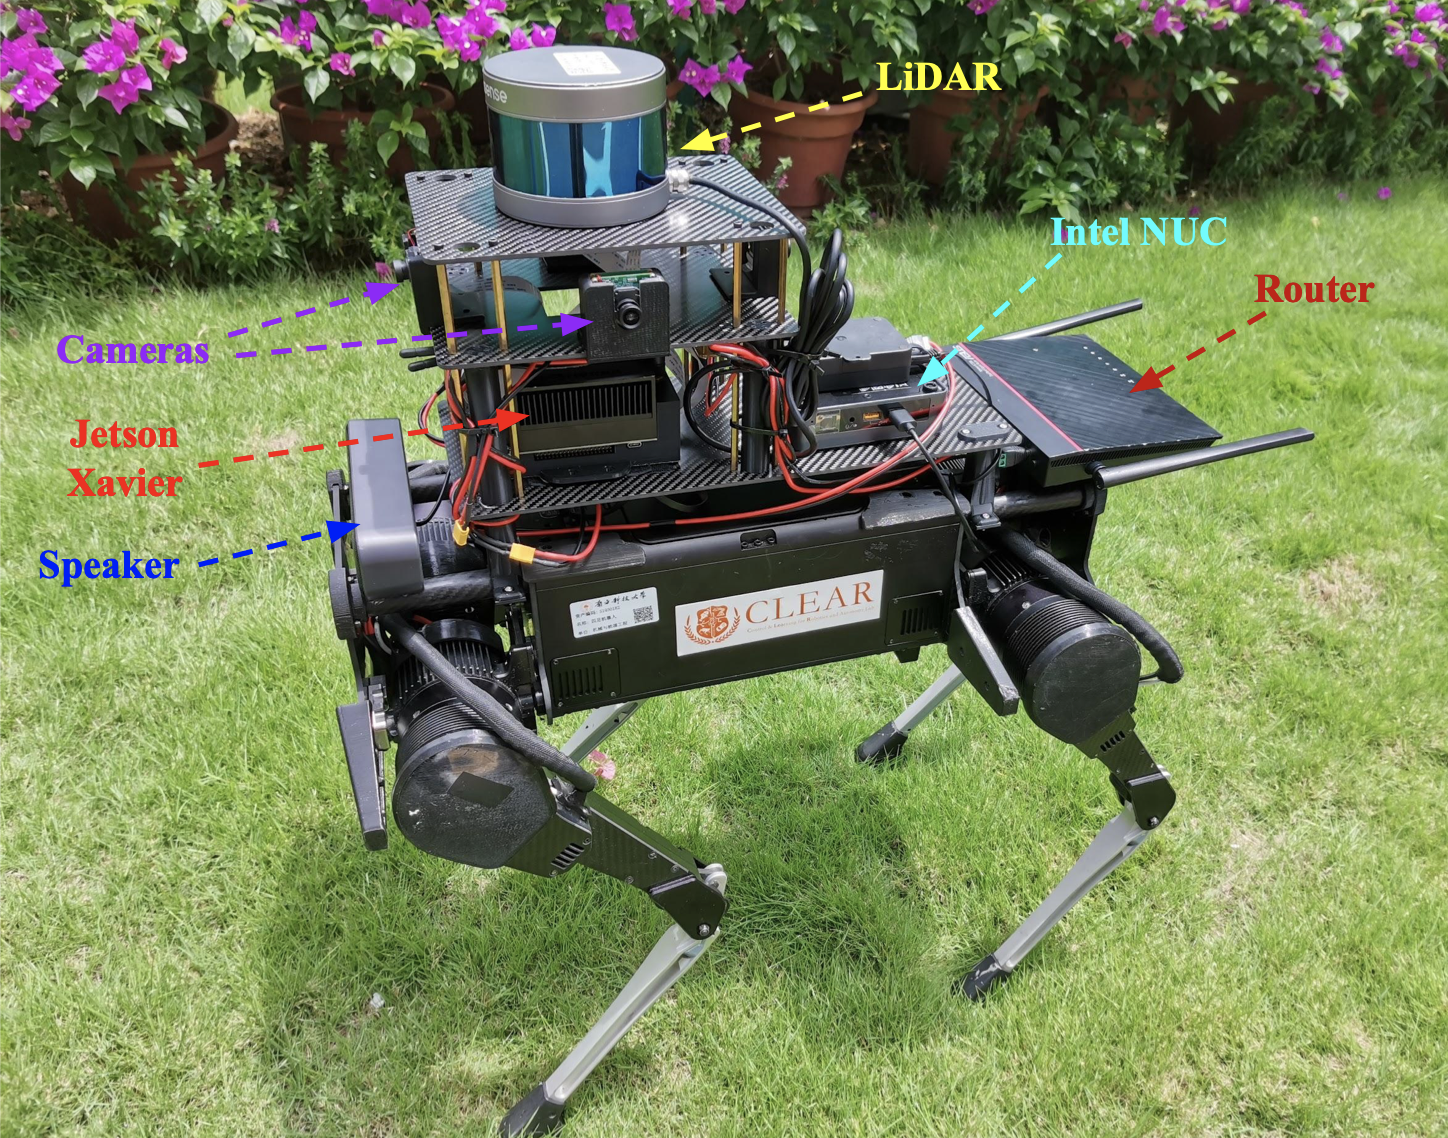
\includegraphics[width=0.8\linewidth]{./img/State_of_art_2.png}
		\end{subfigure}
	\end{figure}
	
	\end{frame}
	
	\begin{frame}{Setup}
	\centering
	\begin{tabular}{|l|l|}
		\hline
		\multirow{2}{4em}{OS} & Ubuntu 18.04 \\
							  & Ubuntu 20.04 \\ \hline
		\multirow{2}{6em}{ROS version} & melodic \\
									   & noetic \\ \hline
		Webots	& R2020b revision 1\\ \hline
		OpenCV~\cite{opencv} 	& 4.x \\\hline
		Imutils~\cite{imutils} & 0.5.3 \\\hline
		Matplotlib~\cite{matplotlib} & 3.3.3 \\\hline
		Numpy~\cite{numpy} & 1.17.2 \\\hline
		Scikit-learn~\cite{scikit} & 0.21.3\\\hline
		{Target hardware}  & Raspberry Pi 3B+ \\ \hline
	\end{tabular}
	\end{frame}


	\section{Gestione dei nodi ROS}\label{sec:Ros}
	\frame{\sectionpage}

	\frame{\begin{figure}[H]
		\centering
		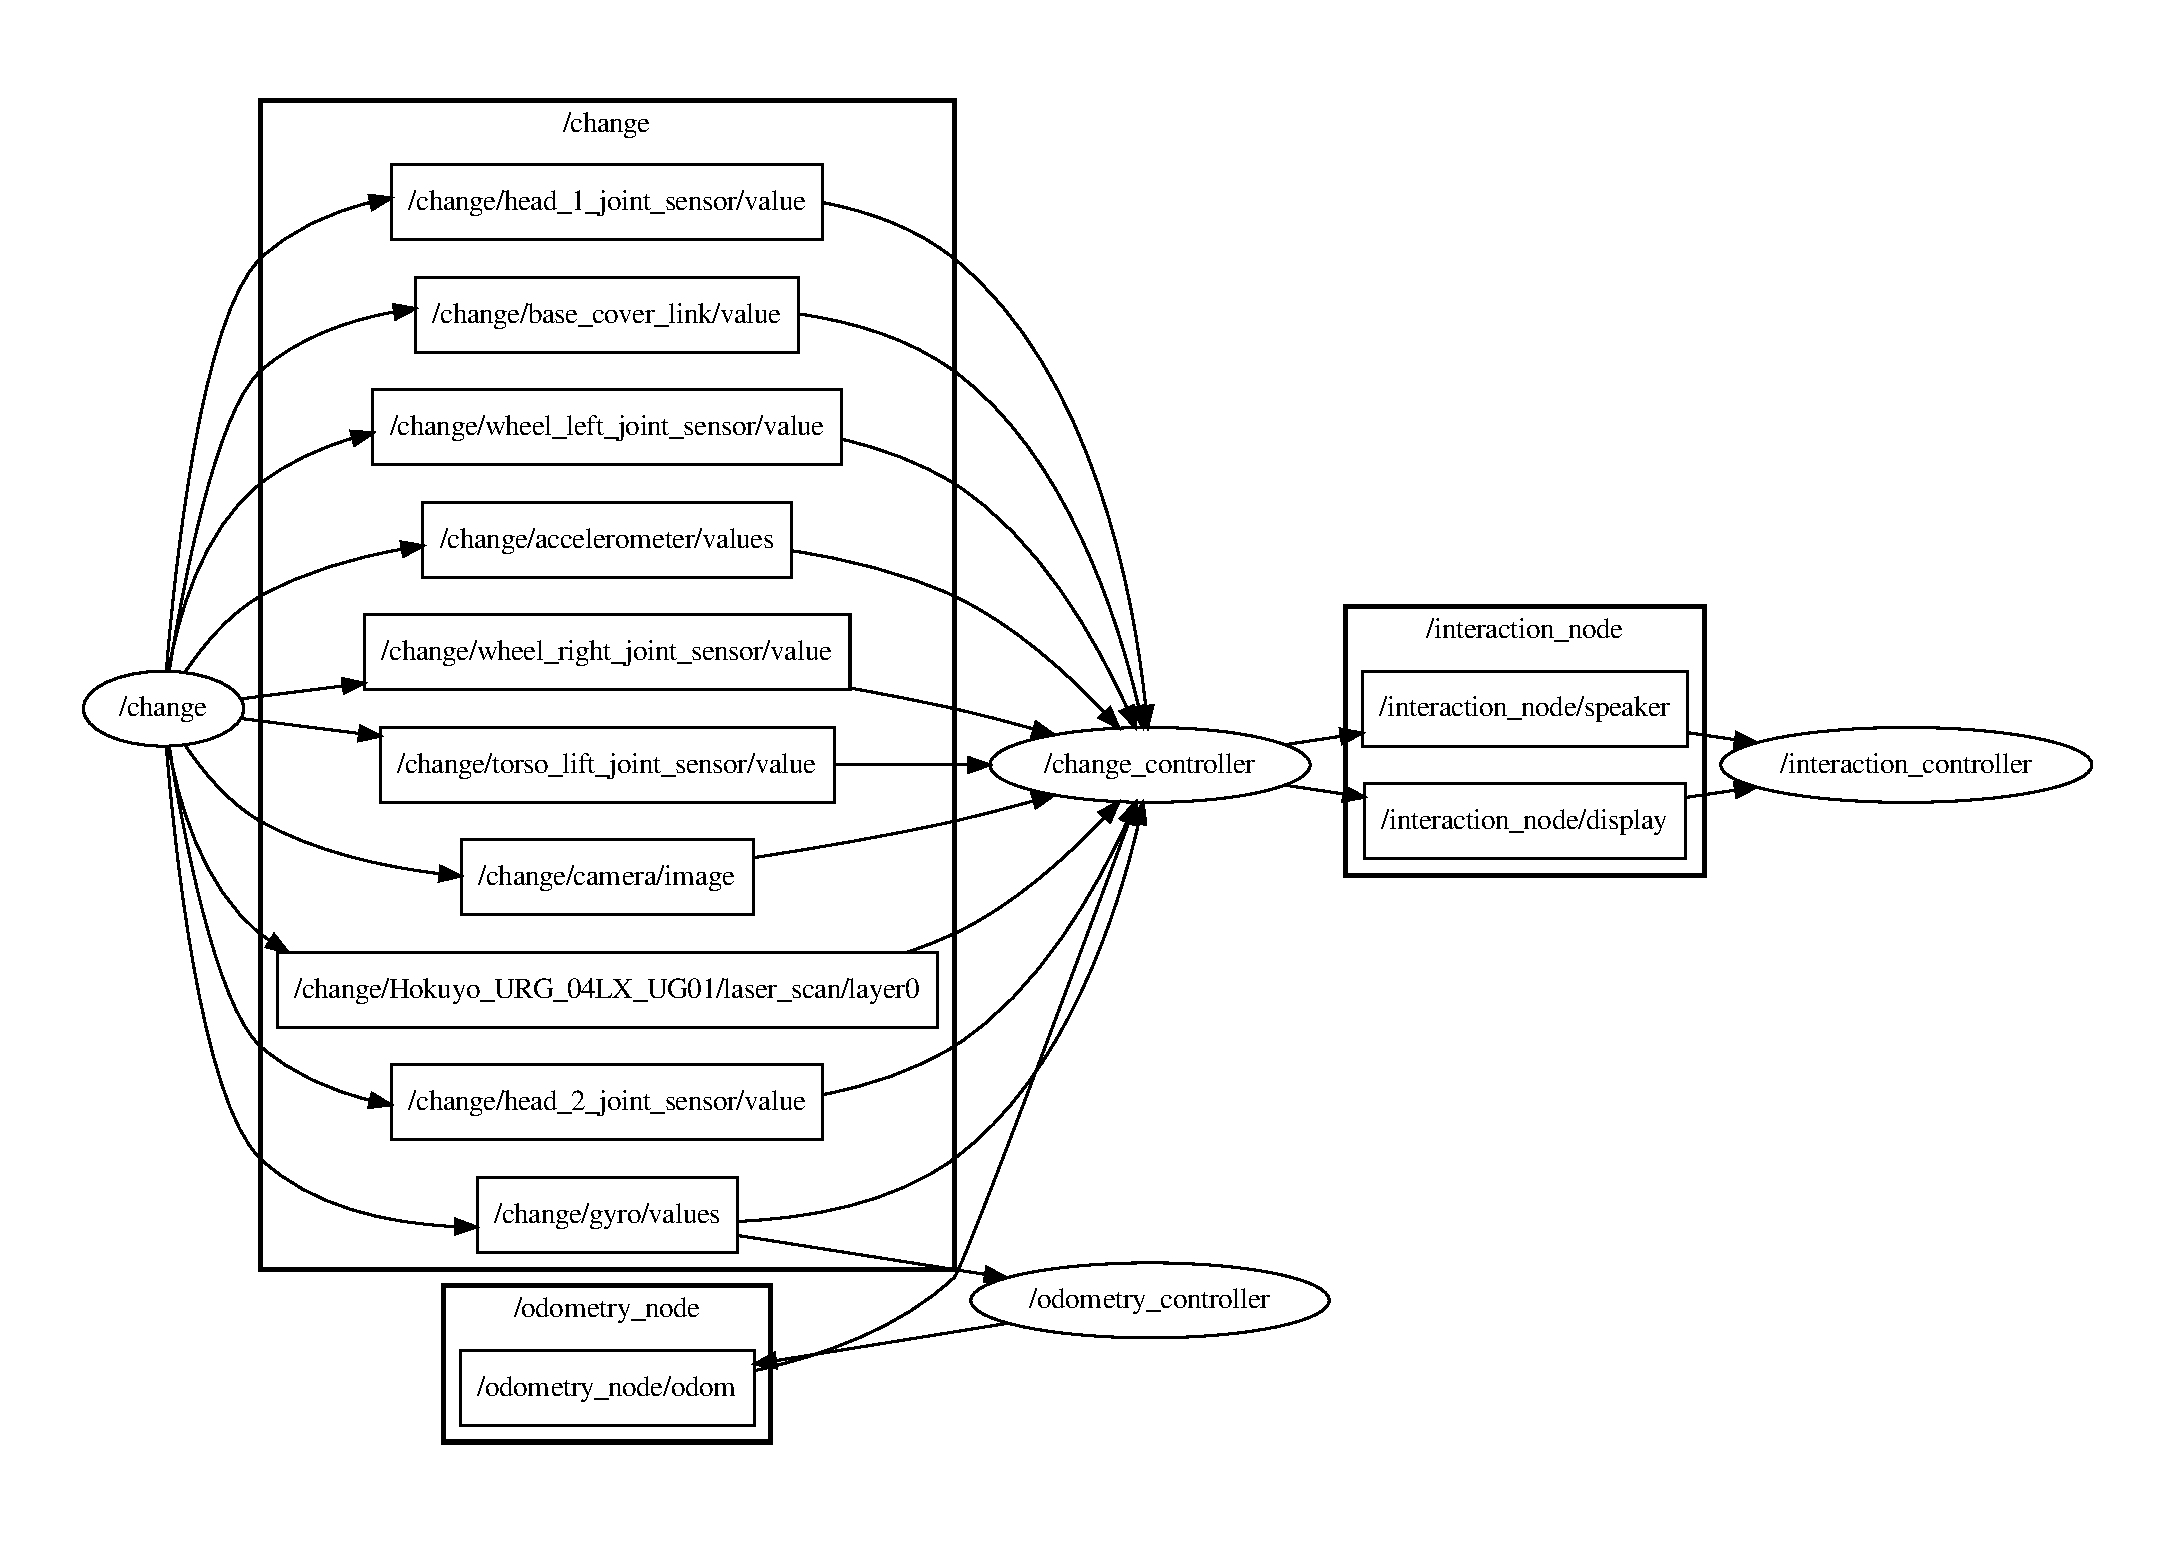
\includegraphics[width=1\textwidth]{img/rosgraph.pdf}
		\caption{Architettura dei nodi ros, ottenuta tramite \textit{rqt}}
		\label{fig:rosgraph}
	\end{figure}
	}

	\begin{frame}{Webots node}
	Questo nodo si occupa solamente di lanciare Webots, e di impostare il
	valore del clock di ROS in base al tempo della simulazione, in modo da
	potere effettuare le integrazioni del tempo correttamente.
	\end{frame}
	\begin{frame}{Change controller node}
	Questo è il nodo che si occupa della gran parte della elaborazione. Oltre
	ad arbitrare sui comportamenti da assumere, gestisce più moduli che si
	occupano di: 
	\begin{itemize}
		\item acquisire i dati dai sensori
		\item mandare i comandi ai motori
		\item gestire il movimento, quindi rotazioni e traslazioni
		\item acquisire e analizzare le immagini dalla camera
	\end{itemize}
	\end{frame}

	\begin{frame}{Interaction node}
	Questo nodo ha il compito di gestire le interazioni audio/video. Ogni
	messaggio che viene riprodotto, prima in lingua italiana e poi inglese,
	viene anche visualizzato testualmente sullo schermo in italiano, inglese e
	cinese.  I possibili comportamenti assunti dal robot sono:
	\begin{itemize}
		\item Salutare all'avvio
		\item Mostrare sul display immagini che esortano a rispettare il
			distanziamento sociale
		\item Riprodurre un messaggio audio che invita a rispettare il distanziamento sociale quando
			rileva un assembramento o quando scansiona l'ambiente
	\end{itemize}
	\end{frame}

	\begin{frame}{Odometry node}
	Il nodo che si occupa dell'odometria si occupa di stimare la posizione del
	robot, come spiegato approfonditamente nella
	sezione~\ref{sec:Modello-del-moto-e-posizionamento}. In generale ciò che fa
	è integrare costantemente i valori del giroscopio e della velocità delle
	ruote per condividere posizione e orientamento del robot.
	\end{frame}
	
	
	\section{TIAGo Iron}\label{sec:TIAGo-Iron} 
	\frame{\sectionpage}
	\frame{

	\begin{columns}
		\begin{column}{0.7\textwidth}
		\justifying
		Il robot scelto per l'obbiettivo proposto è il \textbf{TIAGo Iron}, un
		robot umanoide a due ruote con torso e testa ma senza braccia articolate \cite{pages2016tiago}.
		
		Il datasheet del \textbf{TIAGo} \cite{tiago_datasheet} indica la presenza di speaker e display, non  presenti nel modello Webots \cite{tiagoiron}, che sono quindi stati aggiunti.
		
		La camera del \textbf{TIAGo} è RGB-D ma il modello Webots ne è sprovvisto, di conseguenza è stata utilizzata una camera monoscopica RGB. 
		
		L'IMU utilizzata ha 6 gradi di libertà. 
		
		Il modello Webots del \textbf{TIAGo} presenta un lidar (Hokuyo URG-04LX-UG01 \cite{lidarspecs}) che, conformemente al datasheet,  ha un range di $5.6\,m$ ed un FOV di $240^{\circ}$ (agli estremi è parzialmente occluso).
		\end{column}
		
		\begin{column}{0.3\textwidth}
			\begin{figure}[htpb]
				\centering
				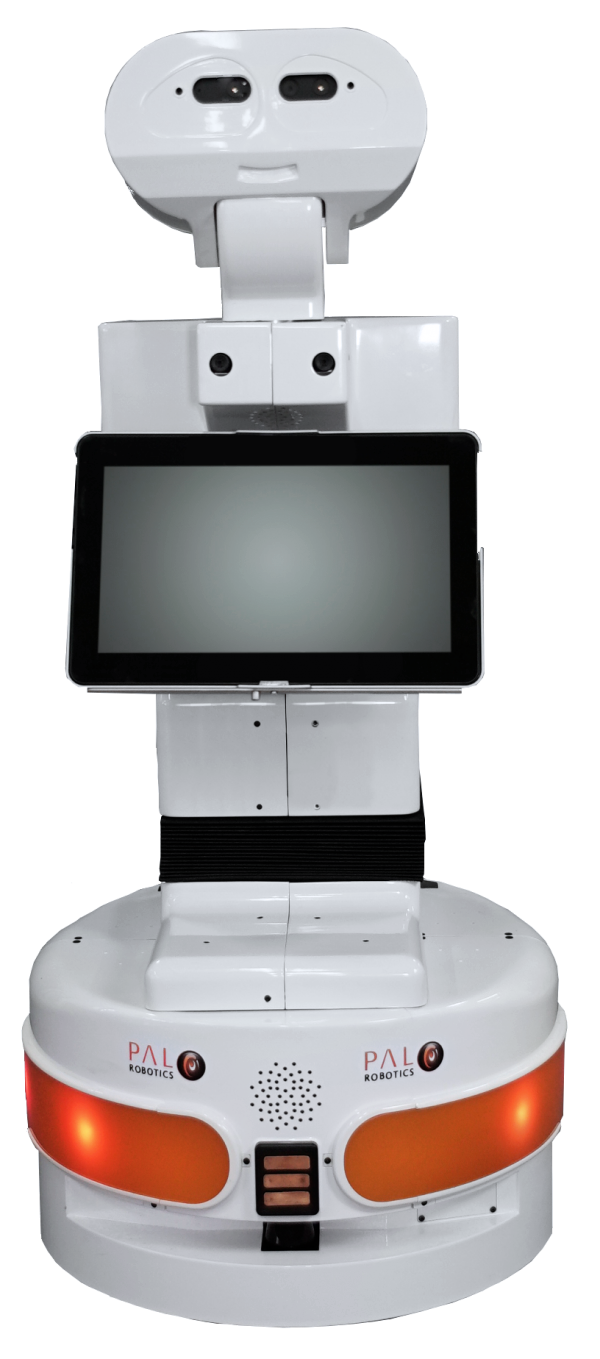
\includegraphics[width=\textwidth]{./img/tiago.png}
				\label{fig:tiago}
			\end{figure}
		\end{column}
	\end{columns}
	
	}

	\section{Modello del moto e posizionamento}\label{sec:Modello-del-moto-e-posizionamento} 
	\frame{\sectionpage}
	
	\begin{frame}{Orientamento}
		Il modello del moto è caratterizzato da rotazioni e traslazioni. Per le
		rotazioni ci basiamo sui dati forniti dal giroscopio, il quale fornisce
		una velocità angolare. Calcoliamo quindi l'angolo di rotazione
		effettuando un'integrazione discreta dei campioni con interpolazione
		lineare del primo ordine (Eq.~\ref{eq:gyro-integration}).  
		\begin{equation}\label{eq:gyro-integration}
			\theta_i = \sum_{j=1}^i \frac{\omega _{j-1}+\omega _j}{2} \left( t_j-t_{j-1} \right) 
		\end{equation}
		Noto l'angolo corrente e l'angolo target utilizziamo un controllore
		proporzionale per raggiungere l'angolo desiderato.
	\end{frame}
	
	\begin{frame}{Spostamento}
		Per effettuare lo spostamento lineare utilizziamo il controllore PID
		
		(Proporzionale-Integrale-Derivativo) delle ruote fornito da Webots, che
		richiede un angolo di rotazione target per ogni ruota. Utilizziamo quindi
		l'angolo di rotazione corrente, e il diametro delle ruote per calcolare la
		posizione delle ruote necessaria al fine di ottenere lo spostamento
		desiderato (Eq.~\ref{eq:odometry}).
		\begin{equation}\label{eq:odometry}
		targetAngle =
		currentAngle+2\pi\frac    {distance}
						{2\pi \cdot diameter}
		\end{equation}
	\end{frame}
	
	\subsection{Posizionamento}\label{subsec:Posizionamento}
	\begin{frame}{Posizionamento}
		Inizialmente al segnale dell'accelerometro
		veniva applicato un integrale doppio per ottenere lo spostamento
		lineare(Eq.~\ref{eq:accel-integration} 	\cite{positioning}).
		
		\begin{equation}\label{eq:accel-integration}
			\begin{cases}
				\textbf{v}_i & = \sum_{j=1}^{i} \frac{\textbf{a} _{j-1}+\textbf{a} _j}{2} \left( t_j-t_{j-1} \right) \\
				\textbf{s}_i & = \sum_{j=1}^{i} \frac{\textbf{v} _{j-1}+\textbf{v} _j}{2} \left( t_j-t_{j-1} \right) 
			\end{cases}
		\end{equation}
		
		Abbiamo ritenuto necessario cambiare approccio, decidendo di utilizzare gli
		encoders delle ruote per determinare gli spostamenti. 
		
		Integriamo la velocità lineare del robot, calcolata a
		partire dal raggio R e le velocità angolari $u[t]$ delle ruote.
		
		\begin{equation}\label{eq:linear-velocity}
			v_i = \frac{R (u_{r,i}+u_{l,i})}{2}
		\end{equation}
		
		Questi valori sono aggiornati ad ogni intervallo di campionamento utilizzando la velocità lineare e la velocità angolare del robot \cite{572228}.
		
		\begin{equation}\label{eq:position-vector-update}
			\textbf{P}_i = \sum_{j = 1}^{i} \begin{bmatrix}
				 & v_i\cos(\theta_i ) & \\
				 & v_i\sin(\theta_i )
			\end{bmatrix}\cdot (t_j-t_{j-1}) 
		\end{equation}		
		
	\end{frame}
	\begin{frame}
		\begin{figure}[H]
			\begin{subfigure}{0.49\textwidth}
				\centering
				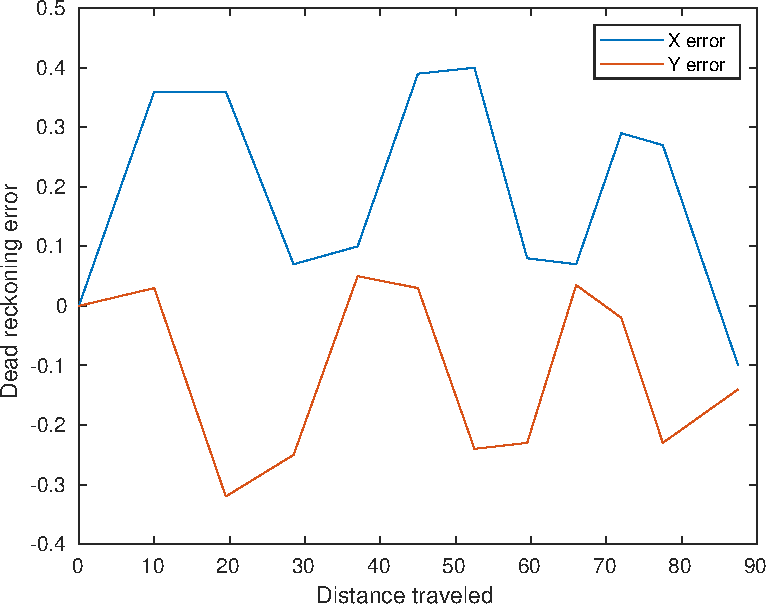
\includegraphics[width=0.8\linewidth]{./img/dead_reckoning_error.pdf}
				\caption{Errore nella stima della posizione}
				\label{fig:dead_reckoning_error}
			\end{subfigure}
			\begin{subfigure}{0.49\textwidth}
				\centering
				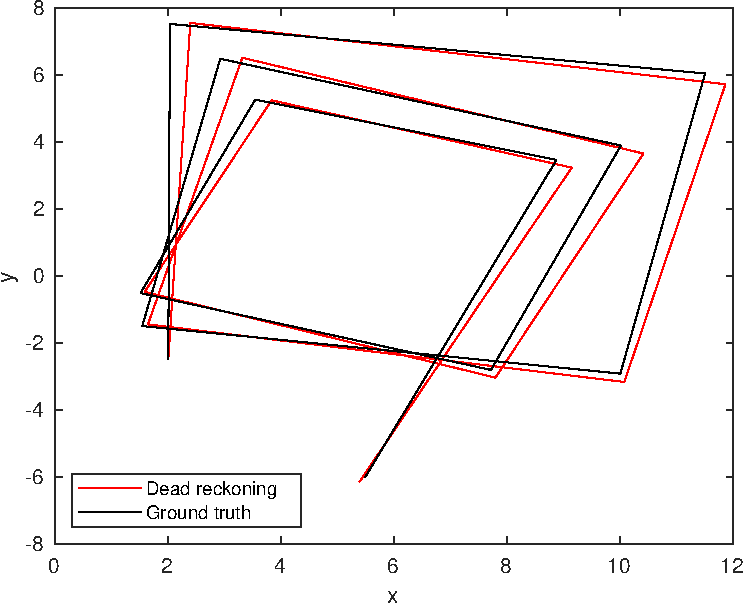
\includegraphics[width=0.8\linewidth]{./img/trajectories.pdf}
				\caption{Errore nella stima della traiettoria}
				\label{fig:trajectory_error}
			\end{subfigure}
		\end{figure}

		Abbiamo misurato le performance della stima di posizione e i risultati
		sono ritenuti soddisfacenti per raggiungere l'obbiettivo proposto.
	\end{frame}
	
	\begin{frame}{Collision avoidance}
		Il \textbf{TIAGo} è in grado di rilevare gli ostacoli grazie
		all'utilizzo di un sensore lidar.  
		
		Nell'immagine seguente viene mostrata la zona nella quale, se viene
		indicata dal lidar la presenza di un ostacolo, il \textbf{TIAGo} si
		ferma per ragioni di sicurezza al fine di evitare danni a persone e/o
		oggetti.
		\begin{figure}[H]
			\centering
			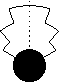
\includegraphics[width=0.2\textwidth]{./img/collision_avoidance.pdf}
			\caption{Collision avoidance}
			\label{fig:collision_avoidance}
		\end{figure}
	\end{frame}
	
	\section{Object recognition}\label{sec:Object-recognition}
	\frame{\sectionpage}
	
	\begin{frame}{Campionamento delle immagini}
		Il FOV della camera è di 57°, quindi per ricoprire 360° è necessario
		effettuare 7 campionamenti. Il settimo campionamento, come si vede in
		figura \ref{fig:campionamento_immagini}, è sovrapposto al primo per 39°.

		È possibile che un individuo si trovi in una zona di confine
		tra due campioni, e che quindi non sia correttamente identificabile in
		nessuna delle due immagini in cui appare parzialmente. Mitighiamo
		questo problema effettuiamo una rudimentale operazione di image
		mosaicing~\cite{ghosh2016survey} e campioniamo l'immagine così
		ottenuta ad intervalli di 28°.
		
		
		\begin{figure}[H]
			\centering
			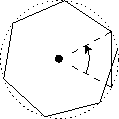
\includegraphics[width=0.3\textwidth]{./img/pictures_sampling.pdf}
			\caption{Campionamento delle immagini}
			\label{fig:campionamento_immagini}
		\end{figure}
	\end{frame}
	
	\begin{frame}{YOLO}
		Abbiamo valutato le performance di
		YOLOv3 (you only look once), YOLOv3-tiny, HoG (Histogram of oriented
		gradients), HoG + SVG (support vector machines).  In seguito a vari test su HoG abbiamo ritenuto essere
		problematica la larghezza delle bounding boxes fornite. YOLOv3 fornisce risultati soddisfacenti.
		
		Considerando le caratteristiche hardware del robot mobile, abbiamo optato per l'uso di
		YOLOv3-tiny, il quale risulta essere significativamente più efficiente
		(approssimativamente del 442\% \cite{tiny_yolo}). Inoltre è rilevante in tal senso un paragone fra YOLOv3 e
		YOLOv3-tiny in termini di mAP (mean average precision) e FLOPS
		(floating-point operations per second) addestrate sul dataset COCO, come
		illustrato dalla tabella.
		
		\begin{table}[htpb]
			\centering
			\begin{tabular}{ |c|c|c|c| } 
				\hline
				Model & mAP & FLOPS & FPS \\
				\hline	
				 YOLOv3-320    & 51.5  &  38.97  Bn  &  45  \\ 
				 YOLOv3-416    & 55.3  &  65.86  Bn  &  35  \\ 
				 YOLOv3-608    & 57.9  &  140.69 Bn  &  20  \\ 
				 YOLOv3-tiny   & 33.1  &  5.56   Bn  &  220 \\
				 YOLOv3-spp    & 60.6  &  141.45 Bn  &  20  \\
				\hline
			\end{tabular}
			\label{tab:comparison}
		\end{table}
		
	\end{frame}

	\section{Posizione dei target}\label{sec:Posizione-dei-target}
	\frame{\sectionpage}
	
	\subsection{Triangolazione}\label{subsec:Triangolazione}
	\begin{frame}{Triangolazione}
		\begin{columns}
			\begin{column}{0.6\textwidth}
				\justifying
				La triangolazione come metodo di individuazione delle persone
				presenta dei problemi nel nostro scenario:
				\begin{itemize}
					\justifying
					\item Occlusione delle persone: se due persone
						(5 e 2) sono una dietro l'altra lungo una retta
						immaginaria che le congiunge al robot (B), quest'ultimo
						non sarà in grado di individuare la più distante. 

					\item Imputazione delle osservazioni: quando il robot
						effettua scan successivi non è in grado di dedurre
						quali osservazioni derivano dalla stessa persona.
						Non è possibile determinare quali intersezioni
						corrispondono ad osservazioni reali e quali sono spurie. 

				\end{itemize}
			\end{column}
			
			\begin{column}{0.4\textwidth}
				\begin{figure}[htpb]
					\centering
					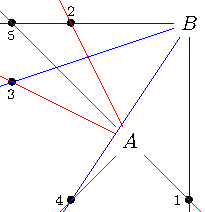
\includegraphics[width=\textwidth]{./img/ideal_object_triangulation.pdf}
					\label{fig:triangulation}
				\end{figure}
			\end{column}
		\end{columns}
	\end{frame}
	
	\subsection{Calcolo della distanza}\label{subsec:Calcolo-della-distanza}
	\begin{frame}[allowframebreaks]{Calcolo della distanza}
		Ipotizzando che la camera abbia un FOV (field of view) di
		$2\alpha$ e sia distante $d$ dall'oggetto, la massima distanza
		orizzontale che un punto dell'immagine potrebbe avere dal centro del
		piano dell'immagine sarebbe $a = d \tan \alpha$.
		
		\begin{figure}[H]
			\centering
			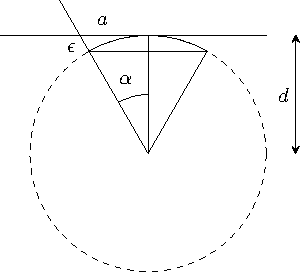
\includegraphics[width=0.4\textwidth]{./img/linearization_error.pdf}
		\end{figure}
		
		Ignorare la prospettiva significa effettuare un'approssimazione lineare
		del primo ordine e trattare il punto come se si trovasse su una
		circonferenza di raggio $d$ centrata sulla camera. Di conseguenza
		consideriamo il punto come se fosse più vicino di quanto non sia
		realmente, commettendo l'errore mostrato nell' Eq.~\ref{eq:max_err}.
		Con una camera con FOV di 1 radiante la sottostima è del 13.9\%.
		
		\begin{gather}
		\begin{aligned}
		\epsilon &= 
		\sqrt{a^2+d^2} - d =
		\sqrt{(d\tan \theta )^2+d^2}-d =\\
		&=d\left( \sqrt{\frac{1}{\cos ^2 \alpha}}-1 \right) =
		d \left( \sec \alpha -1 \right) 
		\end{aligned}
		\label{eq:max_err}
		\end{gather}
		
		\framebreak
		
		Poiché stiamo utilizzando un simulatore non è nota la larghezza del
		sensore da utilizzare per l'eq.~\ref{eq:obj_dist}. Abbiamo ovviato a
		tale problema posizionando il robot ed un oggetto dalle dimensioni note
		in posizioni note e abbiamo utilizzato questi dati insieme a delle
		misure in pixel nell' eq.~\ref{sensor_size}. Abbiamo così stimato le
		dimensioni del sensore virtuale da utilizzare nei calcoli successivi.
		
		\begin{equation}\label{eq:obj_dist}
		object~distance(m) = 
		\frac{f(m) \times real~width(m) \times image~width(pixels)}
		{object~width(pixels) \times sensor~width(m)}
		\end{equation}
		
		\begin{equation}\label{sensor_size}
		sensor~width(m) = 
		\frac{f(m) \times real~width(m) \times image~width(pixels)}
		{object~width(pixels) \times object~distance(m)}
		\end{equation}

	\end{frame}
	
	\subsection{Scarto dei duplicati}\label{subsec:Scarto-dei-duplicati}

	\begin{frame}[allowframebreaks]{Scarto dei duplicati}
		È stato necessario effettuare una fase di clustering al fine di
		scartare le bounding box duplicate. L'algoritmo di clustering
		utilizzato è DBSCAN (Density based scan) \cite{dbscan}, i cui parametri
		principali sono \textbf{eps}, ovvero la massima distanza fra due punti
		affinché vengano considerati appartenenti a un cluster ,
		\textbf{min\_samples}, ovvero il numero minimo di punti affinché un
		cluster sia valido (nel nostro caso è uguale a 1 in quanto non vogliamo
		scartare ROI) ed infine la metrica di distanza.
		
		\begin{figure}[H]
			\centering
			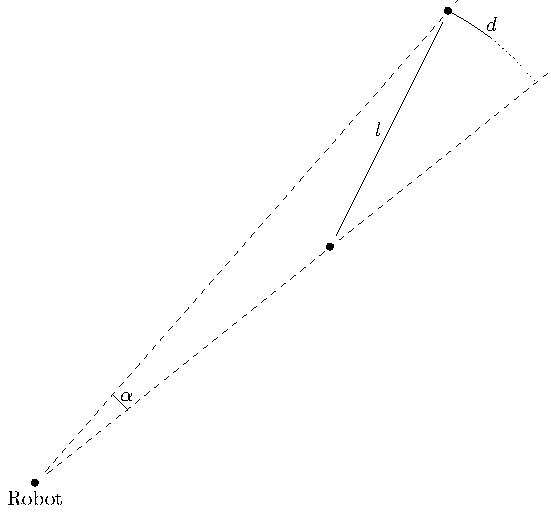
\includegraphics[width=0.4\textwidth]{./img/nms.pdf}
		\end{figure}
	\end{frame}

	\subsection{Correzione dei valori}\label{subsec:Correzione-dei-valori}
	\begin{frame}{Correzione dei valori}
		Per migliorare la stima sulla distanza abbiamo paragonato le reali
		distanze dei target con le stime effettuate dal sistema ottenendo il
		polinomio interpolante $0.003116*x^5 - 0.09722*x^4 + 1.124*x^3
		-5.908*x^2 + 14.5*x-7.367$, che approssima la funzione di correzione della stima. 
		
		\begin{figure}[H]
			\centering
			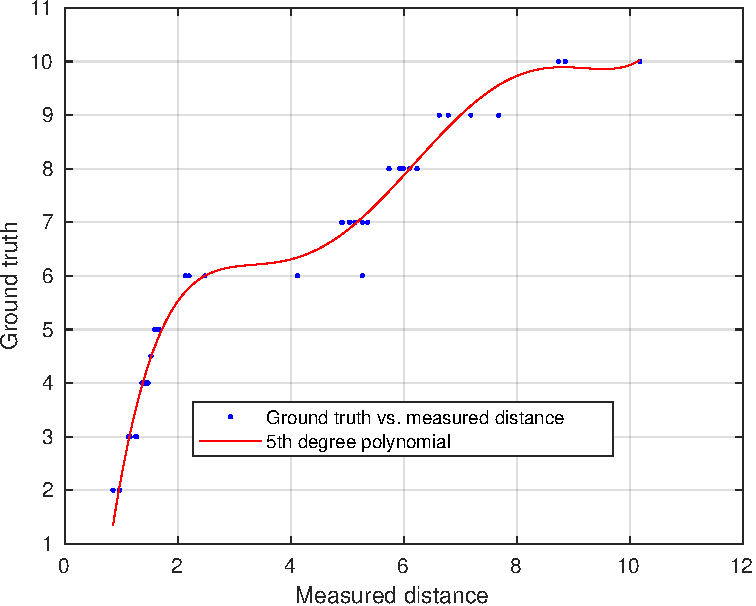
\includegraphics[width=0.7\textwidth]{./img/interpolation.pdf}
			\label{fig:interpolation}
		\end{figure}
	\end{frame}

	\frame{
	Le bontà della stima della distanza e dell'angolo si evince dalle figure :

	\begin{figure}[ht]
		\begin{subfigure}{.49\textwidth}
			\centering
			% include first image
			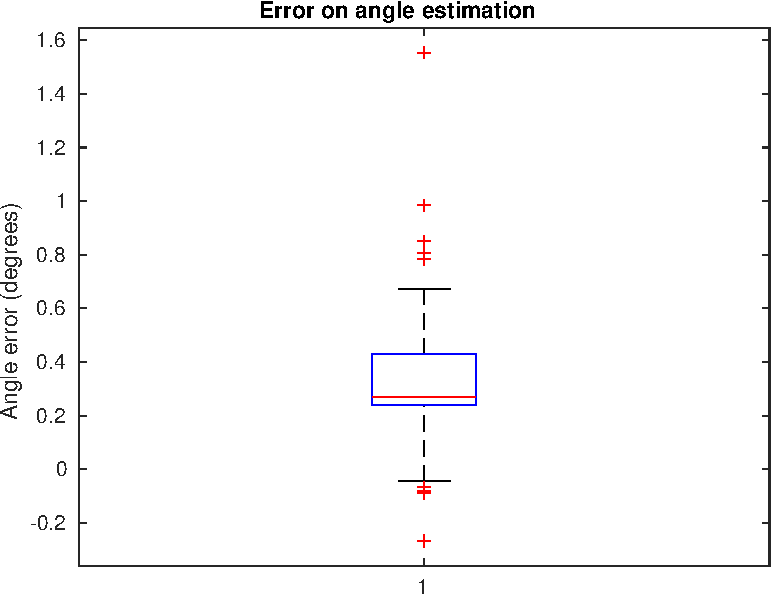
\includegraphics[width=1\linewidth]{./img/angle_error.pdf}  
			\label{fig:angle_plot}
		\end{subfigure}
		\begin{subfigure}{.49\textwidth}
			\centering
			% include second image
			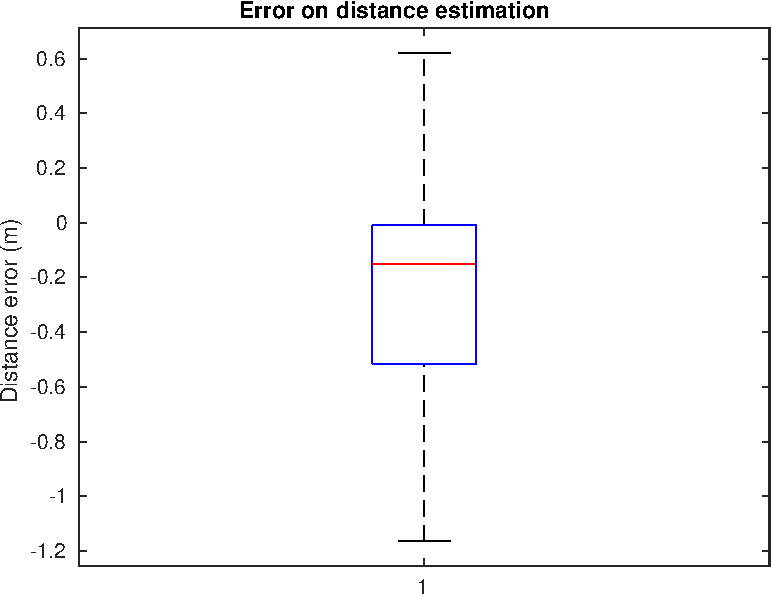
\includegraphics[width=1\linewidth]{./img/distance_error.pdf}  
			\label{fig:distance_plot}
		\end{subfigure}
		\caption{Box plot relativi all'errore su angolo e distanza}
		\label{fig:boxes_plot}
	\end{figure}
	}

	\frame{
	Nelle figure viene riportata la distribuzione gaussiana multivariata rispettivamente in 3 e 2 dimensioni :
	\begin{figure}[H]
		\begin{subfigure}{0.49\linewidth}
			\centering
			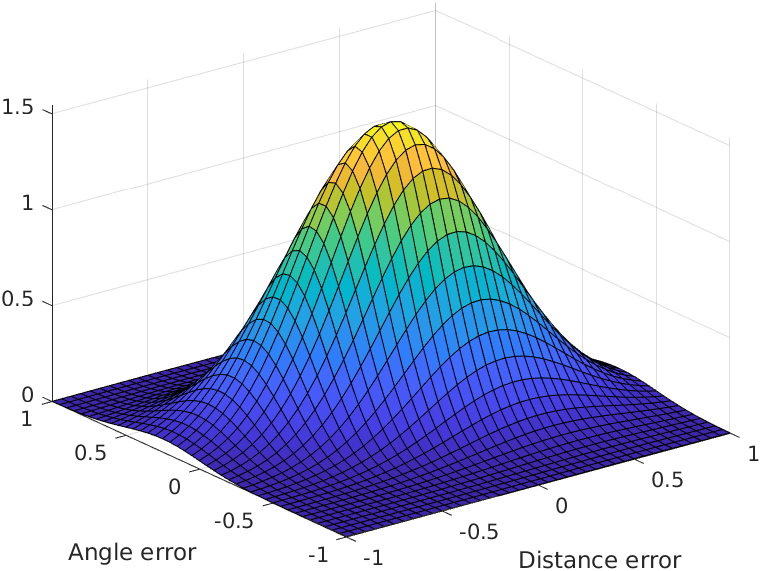
\includegraphics[width=\textwidth]{./img/error_covariance.png}
			\label{fig:error_covariance}
		\end{subfigure}
		\begin{subfigure}{0.49\linewidth}
			\centering
			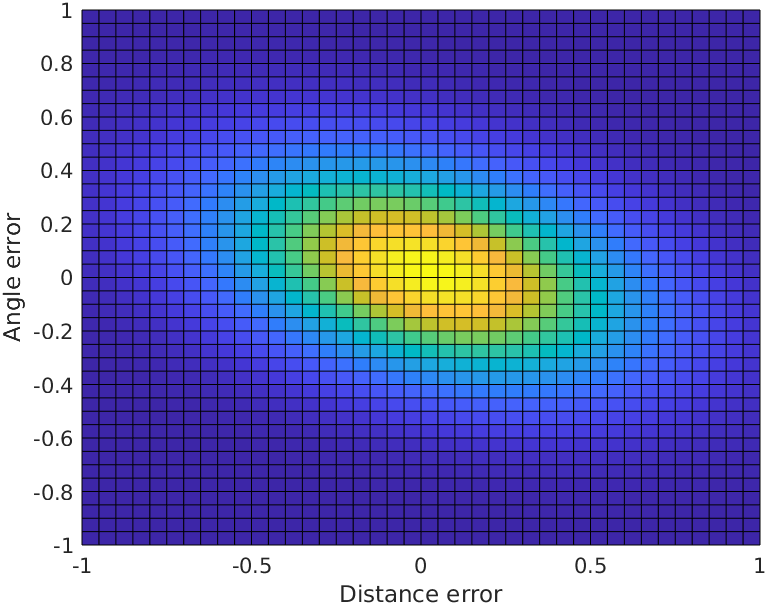
\includegraphics[width=\textwidth]{./img/error_covariance_flat.png}
			\label{fig:error_covariance_flat}
		\end{subfigure}
\end{figure}}
	
	
	\subsection{Modello probabilistico}\label{subsec:Modello-probabilistico}
	Nella nostra applicazione la distanza stimata
	dell'oggetto sarà soggetta ad errore non trascurabile. Per questa
	ragione e per i problemi legati alla triangolazione abbiamo abbandonato la
	rappresentazione basata su oggetti e abbiamo fatto ricorso ad un filtro di
	occupazione bayesiano (BOF)~\cite{tay2008bayesian}.

	Nel filtro di occupazione bayesiano, il problema dell'associazione dei dati viene superato in quanto
	viene gestito da un livello di astrazione superiore. Il concetto di oggetto
	viene difatti riformulato da proprietà più utili quali occupazione o
	rischio, che vengono stimate direttamente per ogni cella utilizzando sia
	osservazioni dai sensori che conoscenze pregresse. Le caratteristiche di
	incertezza legate ai sensori vengono descritte, in questo modello,
	attraverso le probabilità di occupazione.

	Al fine di trasformare le osservazioni ottenute in una probabilità che le
	persone si trovino effettivamente nella posizione indicata è stato
	necessario definire una funzione densità di probabilità. La distribuzione
	normale, sebbene relativamente appropriata nel nostro scenario, è
	computazionalmente onerosa. La griglia di occupazione ha diverse migliaia
	di celle per cui va calcolata una pdf per ogni osservazione. Come si evince
	dalla fig.~\ref{fig:pdf_benchmark} con un numero così elevato di iterazioni
	i tempi di esecuzione non sarebbero accettabili, è stato quindi necessario
	ricorrere ad una approssimazione.
	
	\begin{figure}[H]
		\centering
		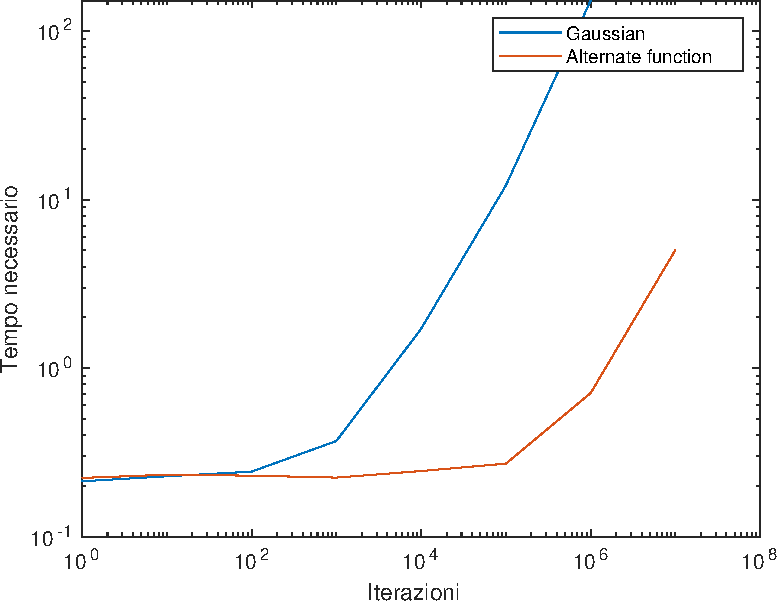
\includegraphics[width=0.6\textwidth]{./img/pdf_benchmark.pdf}
		\caption{Benchmark funzione densità di probabilità (probability density function, funzione )}
		\label{fig:pdf_benchmark}
	\end{figure}

	Un'approssimazione di largo uso è la distribuzione triangolare.
	Quest'ultima, tuttavia, presenta delle caratteristiche non desiderabili per
	il nostro caso d'uso. Una proprietà desiderabile della nostra funzione,
	difatti, sono le "fat tails", ovvero le code della distribuzione devono
	essere spesse e la distribuzione non deve tagliare nettamente. Quando, in
	seguito ad un'osservazione, non abbiamo alcuna osservazione di conferma
	nello scan successivo, non è infatti desiderabile che la probabilità di
	trovare una persona in quel punto scenda a zero. Inoltre, in una prima
	osservazione, un oggetto potrebbe essere occluso ed essere rilevato solo
	successivamente, quindi se in quella zona la probabilità di rilevare un
	target scendesse a zero non sarebbe possibile integrare correttamente
	questa nuova informazione. Ulteriori complicazioni sorgerebbero in caso di
	target in movimento.
	
	Essendo la scansione una operazione estremamente costosa non è nemmeno
	possibile affidarsi esclusivamente all'aggiunta di rumore alla griglia di
	occupazione confidando in una eventuale convergenza.

	Al fine di ottene un'approssimazione di una gaussiana adatta al
	nostro scenario, per modellare la probabilità che data l'occupazione della
	cella in posizione $ {\bf x} $ si ottenga l'osservazione $ {\bf z} $ è
	stato utilizzato un funzionale ispirato al guadagno del filtro di
	Butterworth.
	\begin{equation}\label{eq:pdf}
		p({\bf z}|{\bf x}) = \frac	{K}
		{1 + d({\bf x},{\bf z})^4 } 
	\end{equation}
	Nell'equazione~\ref{eq:pdf} è mostrato il funzionale utilizzato. In
	figura~\ref{fig:pdf_shape} si mostra un confronto della forma di questa
	funzione rispetto ad una gaussiana con media nulla e deviazione standard
	unitaria nel caso monodimensionale.
	
	\begin{figure}[H]
		\centering
		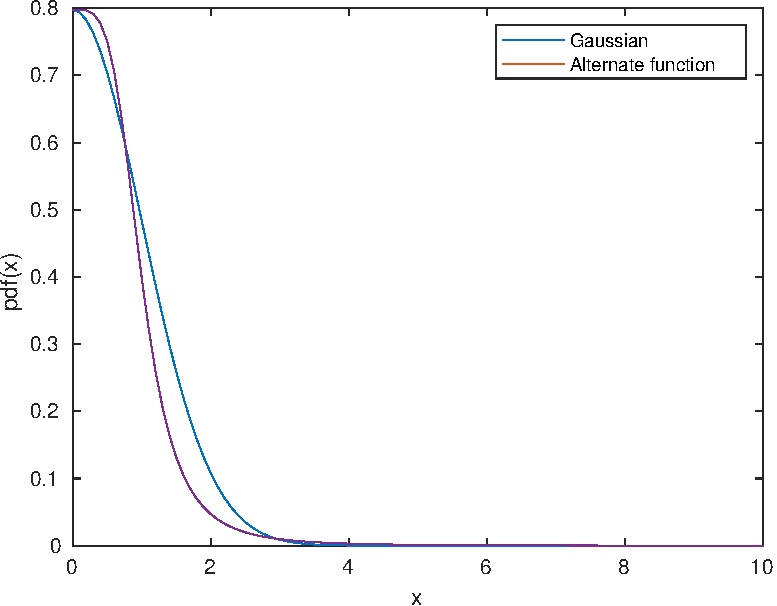
\includegraphics[width=0.6\textwidth]{./img/pdf_shape.pdf}
		\caption{Forma pdf}
		\label{fig:pdf_shape}
	\end{figure}

	Nell'equazione~\ref{eq:pdf} $K$ indica un parametro di scala per ottenere
	CDF unitaria. $d$ è una funzione per il calcolo della distanza della cella
	$ {\bf x} $ dalla stima di posizione $ {\bf z} $.

	La distanza euclidea porterebbe a formare aree ad alta probabilità di forma
	circolare. Questo però non si adatta bene al nostro modello di errore del
	sensore: l'angolo dell'oggetto rispetto al robot è noto con una precisione
	molto elevata, mentre la maggior parte dell'incertezza si concentra nella
	distanza. Calcoliamo quindi la distanza non come distanza euclidea tra le
	coordinate cartesiane della cella e dell'osservazione, ma come norma $ L^2
	$ delle coordinate polari, opportunamente normalizzate per tenere conto
	della diversa incertezza sulla misura di angolo e distanza.

	L'incertezza sulla distanza è ricavata dalle misure di calibrazione
	effettuate. Per l'angolo è stato seguito un approccio differente:
	utilizzare una varianza calcolata a partire da una serie di osservazioni
	porterebbe ad assegnare maggiore probabilità ad oggetti lontani.  In un
	setup come quello in figura~\ref{fig:circular_sector}, con due target
	rilevati, rispettivamente a distanza $d_1$ e $d_2$, le aree ad alta
	probabilità relative ad entrambi i punti avranno lunghezza $l$ e ampiezze $
	\alpha_1 \text{ e } \alpha_2  $. 
	
	\begin{figure}[H]
		\centering
		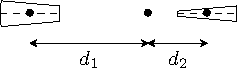
\includegraphics[width=0.5\textwidth]{img/circular_sector.pdf}
		\caption{Area della regione probabile a seconda della distanza.}
		\label{fig:circular_sector}
	\end{figure}

	Come mostrato nell'equazione~\ref{eq:circular_sector}, con queste
	condizioni la dimensione dell'area ad alta probabilità è direttamente
	proporzionale alla distanza e all'ampiezza dell'angolo. Se quindi $
	\alpha_1 $ coincidesse con $ \alpha _2 $ ad oggetti distanti verrebbero
	associate aree molto più grandi. 

	\begin{subequations}\label{eq:circular_sector}
	\begin{align*} 
		A_1  = & \pi((d_1+l/2)^2-(d_1-l/2)^2)\frac{\alpha_1}{2\pi}  =  \alpha_1 d_1l \\
		A_2  = & \pi((d_2+l/2)^2-(d_2-l/2)^2)\frac{\alpha_2}{2\pi}  =  \alpha_2 d_2l \\
\tag{\ref{eq:circular_sector}}
		\frac{A_1}{A_2} = & \frac	{\alpha_1 d_1} {\alpha_2 d_2}
	\end{align*}
	\end{subequations}
	
		
	Per evitare questo problema, dopo avere
	individuato un valore $ \alpha ^* $ appropriato questo viene scalato per un
	coefficiente inversamente proporzionale alla distanza della cella, quindi $
	\alpha _1 = \alpha ^*/d_1 $ e $ \alpha _2=\alpha ^*/d_2 $, da cui $A_1=A_2$. 
	
	Questa misura di distanza è in accordo con l'intuizione derivata dal fatto
	che un oggetto più lontano occuperà una porzione più piccola dell'immagine,
	di conseguenza ci sono meno posizioni valide che la ROI associata
	all'oggetto può assumere, e quindi l'intervallo di valori che può assumere
	l'angolo è ridotto.

	
	Dato un insieme di osservazioni ottenute da una scansione $ Z_i $ aggiorniamo il belief precedente rispetto ad ogni cella della griglia di occupazione come mostrato nell'equazione~\ref{eq:belief-update}.

	\begin{equation}\label{eq:belief-update}
		p({\bf x}_i | Z_i) = p({\bf x}_{i-1}) \cdot 
		\sum_{{\bf z} \in Z_i} p({\bf z} | {\bf x})
	\end{equation}
	Al termine di ogni aggiornamento della mappa l'intera griglia viene inoltre
	normalizzata per avere somma unitaria.  
	Questa formula è valida sotto le seguenti assunzioni:
	\begin{itemize}
		\item In uno stesso scan osservazioni separate si riferiscono ad
			oggetti distinti. In altre parole date due osservazioni $z_1$ e
			$z_2$ queste non hanno intersezione, quindi $ p(z_1 \cup z_2) =
			p(z_1)+p(z_2)-p( z_1 \cap z_2) = p(z_1)+p(z_2) $ 

			Questa assunzione è ragionevole ricordando che lo scan avviene
			ruotando intorno al centro del robot e che viene effettuato uno
			scarto dei duplicati tenendo conto dell'angolo, quindi non possono
			esserci due osservazioni distinte derivanti dall'occupazione della
			stessa posizione nella mappa.

		\item In assenza di nuove osservazioni la stima dello stato del sistema
			rimane invariata: $ \overline{bel}(x_i) = bel(x_{i-1}) $ 

			Il robot non si muove abbastanza velocemente da poter inseguire e
			raggiungere assembramenti di breve durata, ha senso quindi
			limitarsi a considerare situazioni prevalentemente stazionarie e
			assumere consistenza dell'ambiente tra uno scan e l'altro. Inoltre
			gli scan sarebbero comunque troppo infrequenti per ottenere stime
			significative sul movimento degli oggetti.

	\end{itemize}

	In pratica applicando direttamente queste formule si introdurrebbe un
	errore nell'interpretazione delle informazioni: se per qualche ragione in
	uno scan non venisse rilevato nessun oggetto, $ Z_i $ sarebbe l'insieme
	vuoto. In mancanza di nuovi dati si potrebbero tentare due approcci:
	resettare le stime o lasciarle del tutto invariate. Nessuno di questi
	approcci si dimostra soddisfacente:
	\begin{itemize} 
		\item Lasciare invariato il belief a seguito di multiple scansioni
			senza successo porterebbe a non notare che tutte le persone
			nell'ambiente in cui ci si trova sono andate via, continuando a
			considerare valide tutte le posizioni precedenti.
		\item Dall'altro lato, un approccio troppo drastico quale
			immediatamente scartare tutte le precedenti stime porterebbe a
			perdere informazioni utili a causa di occlusioni temporanee (e.g.
			il robot entra in una stanza vuota).
	\end{itemize}

	Per gestire questa situazione effettuiamo uno smoothing degli istogrammi
	prima di ogni update essendoci una diminuzione della certezza delle misure.
	Aggiungiamo inoltre del rumore. In questo modo in assenza di osservazioni
	ci sarà una tendenza al ritorno ad uno stato iniziale, ma sarà graduale in
	modo da evitare di scartare troppo rapidamente le informazioni pregresse.

	Al fine di individuare le zone con alta probabilità di contenere persone
	abbiamo utilizzato un approccio derivante dall'elaborazione delle immagini.
	In primo luogo separiamo i punti nella mappa in punti ad alta probabilità
	di essere occupati da persone e punti con bassa probabilità. Per effettuare
	questa sogliatura abbiamo utilizzato il metodo Otsu~\cite{otsu}, il quale
	applica un thresholding automatico calcolato minimizzando la varianza dei
	valori di intensità all'interno delle classi e massimizzandola fra classi
	differenti all'immagine in input.  
	
	Da questa sogliatura otteniamo una mappa binaria in cui sono evidenziate le
	celle ad alta probabilità. Applicando l'algoritmo in~\cite{contours},
	implementato in OpenCV, estraiamo le regioni ad alta probabilità contigue
	ed i loro contorni. Per ogni regione verrà selezionato come centro il punto
	con maggiore probabilità (Fig.~\ref{fig:image_segmentation}).

	\begin{figure}[H]
		\centering
		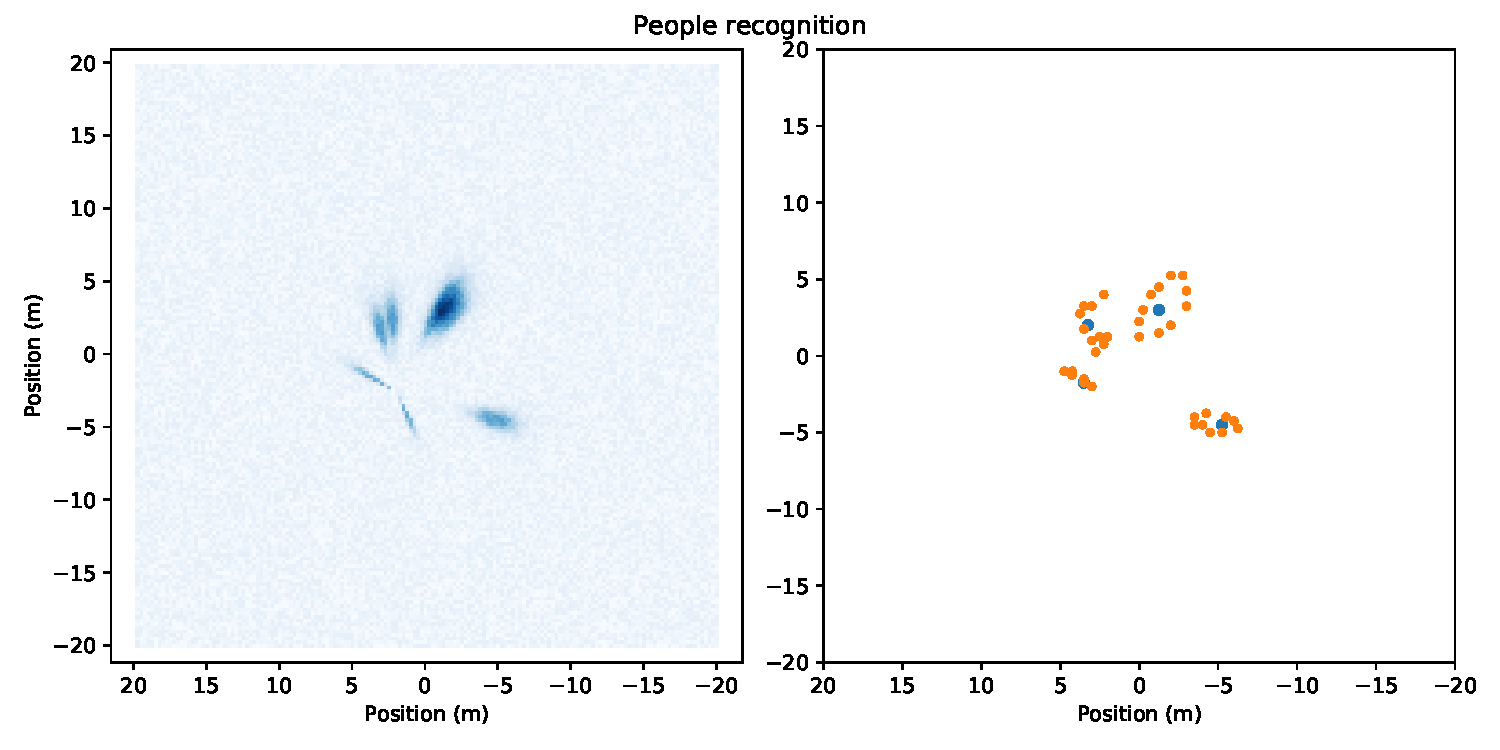
\includegraphics[width=1\textwidth]{./img/image_segmentation.pdf}
		\caption{Segmentazione immagine: a sinistra i valori grezzi del BOF, a destra i contorni delle regioni (giallo) e i centri (blu) }
		\label{fig:image_segmentation}
	\end{figure}

	\section{Pianificazione del moto}\label{sec:Pianificazione-del-moto}
	\frame{\sectionpage}
	
	\subsubsection{Modalità esplorazione}\label{subsec:Modalita-esplorazione}
	\begin{frame}{Modalità esplorazione}
		Quando il robot entra in modalità esplorazione il suo comportamento è
		di esplorazione casuale della mappa. Il robot continua ad esplorare ed
		effettuare scan periodici fino a quando non viene rilevato un
		obbiettivo.  In tal caso il robot entra in modalità campi di
		potenziale. Se il robot incontra un ostacolo nel suo cammino ruota di
		$90^{\circ}$ nella direzione con più spazio e continua l'esplorazione
		casuale.
	\end{frame}
	
	\subsubsection{Bug mode}\label{subsec:Bug-mode}
	\begin{frame}{Tangent bug~\cite{503814}}
		Quando il robot entra in modalità bug effettuiamo uno scan lidar.
		Poiché lavoriamo con valori discreti, confrontiamo i valori ottenuti
		con una soglia al fine di individuare le discontinuità nel profilo
		degli oggetti nel range. Analizziamo le discontinuità
		del segnale per individuare i bordi degli ostacoli
		(Fig.~\ref{fig:bug}). 
		Il robot si muove verso il punto al quale corrisponde l'angolo più
		vicino a quello del target, che ci farà allontanare meno
		dall'obbiettivo.
		
		\begin{figure}[H]
			\centering
			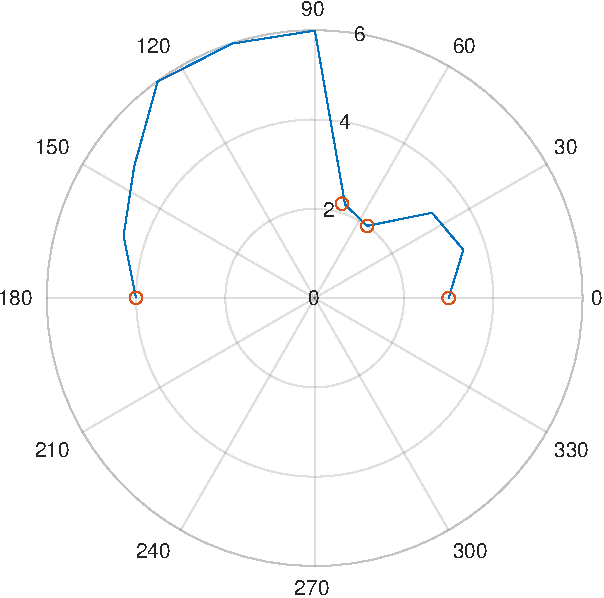
\includegraphics[width=0.4\textwidth]{./img/bug.pdf}
			\caption{Profilo dell'ostacolo}
			\label{fig:bug}
		\end{figure}
	\end{frame}

	\subsubsection{Campi di potenziale}\label{subsec:Campi-di-potenziale}
	
	Una soluzione al classico problema di muoversi in uno spazio evitando le
	collisioni è l'uso di un modello basato sui campi di potenziale. Questi
	schemi richiedono la definizione di potenziali attrattivi e repulsivi.
	Tuttavia, questi metodi presentano una problematica significativa: la
	presenza di un minimo locale causerà una forza totale sul punto nulla, e di
	conseguenza il robot si fermerà in una posizione non ideale. 

	Il potenziale attrattivo è centrato sul target, ed è modellato come un
	potenziale quadratico, la forza attrattiva è quindi lineare rispetto alla
	distanza (Eq.~\ref{eq:attractive-force}).

	Gli ostacoli generano invece un potenziale repulsivo. Questo ha un raggio
	d'azione limitato, la forza repulsiva è massima per un ostacolo a distanza
	nulla, e decresce in modo monotono fino ad annullarsi se la distanza
	dell'ostacolo supera una soglia $d_t$ con la legge descritta
	nell'equazione~\ref{eq:repulsive-force}.

	La maggior parte dei potenziali repulsivi descritti in letteratura
	dipendono esclusivamente dalla distanza dall'ostacolo, interferendo con il
	moto anche se questo avviene parallelamente all'ostacolo. Per ovviare a
	questo problema prendiamo in considerazione solo gli ostacoli situati in un
	FOV frontale al robot con ampiezza $ \alpha  $ calcolata per permettere di
	muoversi parallelamente ad una superficie mantenendo una distanza di
	sicurezza $ h $ (Eq.~\ref{eq:obstacle_fov}, Fig.~\ref{fig:obstacle_fov}): 


	\begin{equation}\label{eq:attractive-force}
		F_{att}( \textbf{x}) = k_a\cdot \left| {\bf x - x_d} \right| 
	\end{equation}

	\begin{equation}\label{eq:repulsive-force}
		F_{rep}(obstacleDistance) = \begin{cases}
			k_r \cdot \left(
				\frac{1}{obstacleDistance^2}-
				\frac{1}{d_t^2}
			\right)  & obstacleDistance \leq d_{t} \\
			0 & d > d_{thresh}
		\end{cases}
	\end{equation}

	\begin{equation}\label{eq:obstacle_fov}
		\alpha = {2}\sin^{-1}{\frac{h}{d_t}}
	\end{equation}

	\begin{figure}[H]
		\centering
		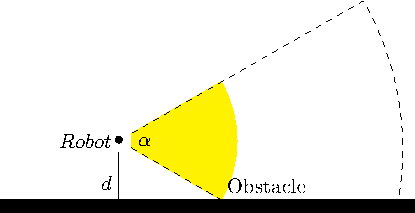
\includegraphics[width=0.8\textwidth]{./img/obstacle_fov.pdf}
		\caption{FOV frontale del robot}
		\label{fig:obstacle_fov}
	\end{figure}

	L'approccio seguito consiste in due comportamenti calcolati
	indipendentemente: il comportamento traslatorio e il comportamento
	rotazionale.

	La traslazione viene calcolata in funzione dello spazio di movimento a
	disposizione e dall'angolo rispetto al target secondo
	l'equazione~\ref{eq:translation}, ottenuta per interpolazione del profilo
	desiderato.

	\begin{equation}\label{eq:translation}
		d = 0.5 + \frac	{0.9\cdot obstacleDistance - 0.5}
		{1 + \left|
				\frac{6\omega}{\pi}
		\right|  } 
	\end{equation}
	
	\begin{equation}\label{eq:angle}
		\omega = \begin{cases}
			\omega^*=\theta - \angle\left( \textbf{F}_{att} - \textbf{F}_{rep} \right)  & -\Omega \le \omega^* \le \Omega \\
			-\Omega & \omega^* < -\Omega \\
			\Omega & \omega^* < \Omega

		\end{cases}	\end{equation}
	
	\subsection{Pianificazione}\label{subsec:Pianificazione}
	\begin{frame}{Scheduling dei comportamenti}
		
		\begin{columns}
			\begin{column}{0.5\textwidth}
				In seguito all'avvio, \textbf{Change} effettua uno scan
				dell'ambiente.  Nel caso in cui non vengano rilevati obbiettivi
				entra in modalità esplorazione e, dopo aver percorso una
				determinata distanza, effettua nuovamente uno scan
				dell'ambiente. Nel caso in cui venga rilevato un obbiettivo il
				robot entra in modalità campi di potenziale e si muove verso
				l'obbiettivo, effettuando nuovi scan nel caso in cui abbia
				raggiunto l'obbiettivo o percorso una determinata
				distanza. Se, in modalità campi di potenziale, il
				\textbf{TIAGo} rimane bloccato in un loop, entra in modalità
				Tangent Bug, fin quando non esce dal loop, e ritorna nella
				modalità campi di potenziale.
			\end{column}
			
			\begin{column}{0.5\textwidth}
				\begin{figure}[H]
					\centering
					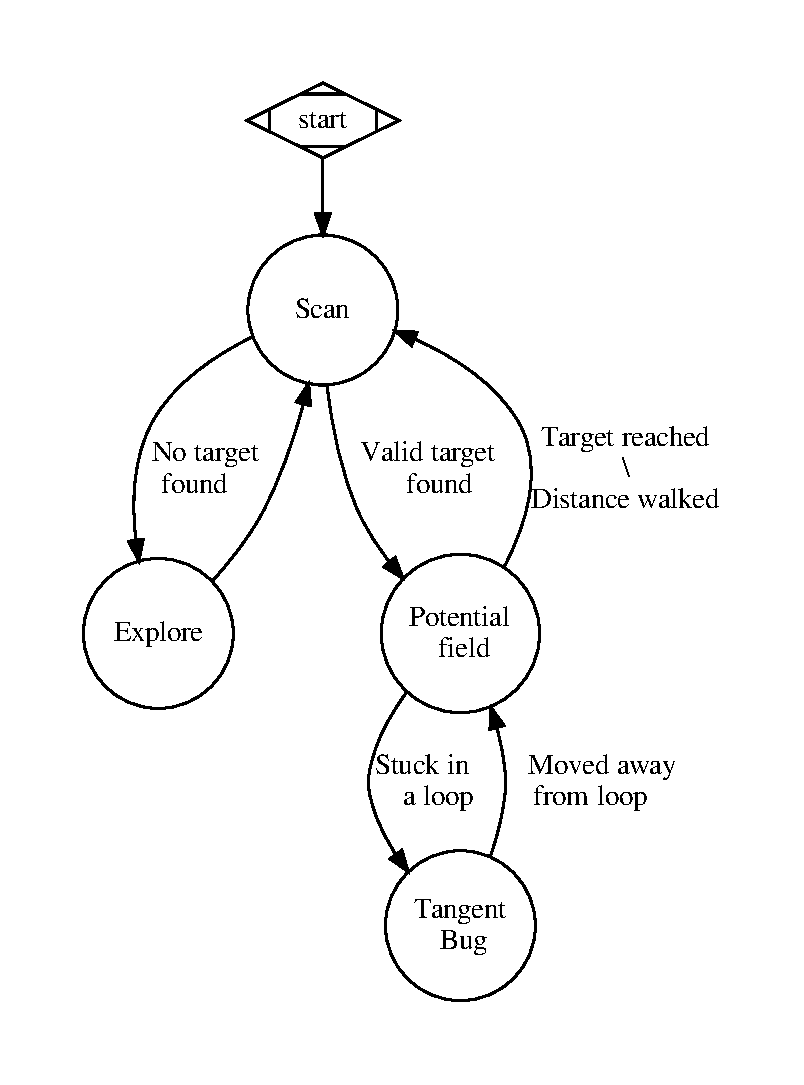
\includegraphics[width=\textwidth]{./img/fsa.pdf}
					\label{fig:fsa}
				\end{figure}
			\end{column}
		\end{columns}
	\end{frame}
	
	\section{Possibili modifiche}\label{sec:Possibli-modifiche}
	\frame{\sectionpage}
	\frame{
		Riportiamo di seguito possibili modifiche da apportare:
		\begin{itemize}
			\item Aggiungere un algoritmo per effettuare SLAM, in modo da poter
				pianificare il moto con algoritmi come A* \cite{A*} o RRT
				\cite{RRT}
			\item Migliorare la modalità Tangent Bug
			\item Utilizzare una depth-cam per stimare con più precisione la
				distanza delle persone
			\item Tracciamento delle persone in real-time
		\end{itemize}
	}

	\newpage
    % Bibliography
	\bibliographystyle{unsrt}
	\begin{frame}[allowframebreaks]{Riferimenti bibliografici}
		\bibliography{references.bib}
	\end{frame}



\end{document}
